\section{Architecture}
\label{sec:architecture}

Since the development of a real botnet goes beyond the scope of this work, we adhere to an architecture that allows us to focus on the development of a bot, thought for testing and educational showcase, but actually ready for a real scenario. \Cref{fig:botnet-architecture} shows our botnet reference architecture.

\begin{figure}[tp]
  \centering
  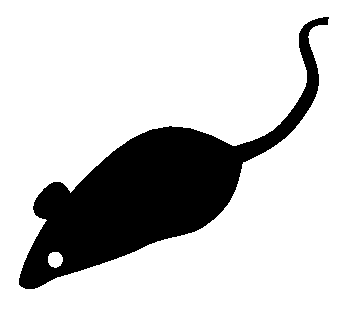
\includegraphics{./fig/acmlarge-mouse}
  \caption{\textcolor{blue}{The botnet architecture. Lorem ipsum dolor sit amet, consectetur adipiscing elit, sed do eiusmod tempor incididunt ut labore et dolore magna aliqua. Ut enim ad minim veniam, quis nostrud exercitation ullamco laboris nisi ut aliquip ex ea commodo consequat. Duis aute irure dolor in reprehenderit in voluptate velit esse cillum dolore eu fugiat nulla pariatur. Excepteur sint occaecat cupidatat non proident, sunt in culpa qui officia deserunt mollit anim id est laborum.}}
    \label{fig:botnet-architecture}
\end{figure}

The reference architecture models a bot that can be instructed by a centralized controller.
Here, a controller is defined giving three interfaces: the \textit{init interface} is the one through wich the bot joins the botnet loading specific configuration; the \textit{command interface} is the one through which the bot loads commands to execute; the \textit{log interface} is the one that the bot submits analysis reports to.

Such a model makes our bot is suitable both for local testing, where interfaces are local files, and real controller interaction, where interfaces are REST interfaces.

Our bot can be configured by a convenient Web User Interface (WUI) described in \Cref{sec:configuration-wui}. The commands it can execute are given as JSON file. These files can be both local files and remote controller responses. They can be conveniently created by a WUI described in \Cref{sec:commands-wui}.
